%%%%%%%%%%%%%%%%%%%%%%%%%
% Dokumentinformationen %
%%%%%%%%%%%%%%%%%%%%%%%%%


%\setDefaultArrayStretch{1}

\newcommand{\titleinfo}{Elektronik 1}
\newcommand{\authorinfo}{Braun, Jürg, Gwerder, Waldvogel, Badertscher \& Co}
\newcommand{\versioninfo}{$Version 1.0$}
% Genereller Header
\documentclass[10pt,twoside,a4paper,fleqn]{article}
\usepackage[utf8]{inputenc}
\usepackage[left=1cm,right=1cm,top=1cm,bottom=1cm,includeheadfoot]{geometry}
\usepackage[ngerman]{babel,varioref}

% Pakete
\usepackage{amssymb,amsmath,fancybox,graphicx,color,lastpage,wrapfig,fancyhdr,hyperref,verbatim}

%%%%%%%%%%%%%%%%%%%%
% Generelle Makros %
%%%%%%%%%%%%%%%%%%%%
\newcommand{\formelbuch}[1]{$_{\textcolor{red}{\mbox{\small{S#1}}}}$}
\newcommand{\verweis}[2]{\small{(siehe auch \ref{#1}, #2 (S. \pageref{#1}))}}
\newcommand{\subsubadd}[1]{\textcolor{black}{\mbox{#1}}}


\newcommand{\skriptsection}[2]{\section{#1 {\tiny Skript S. #2}}}
\newcommand{\skriptsubsection}[2]{\subsection{#1 {\tiny Skript S. #2}}}
\newcommand{\skriptsubsubsection}[2]{\subsubsection{#1 {\tiny Skript S. #2}}}

%%%%%%%%%%
% Farben %
%%%%%%%%%%
\definecolor{black}{rgb}{0,0,0}
\definecolor{red}{rgb}{1,0,0}
\definecolor{white}{rgb}{1,1,1}
\definecolor{grey}{rgb}{0.8,0.8,0.8}

%%%%%%%%%%%%%%%%%%%%%%%%%%%%
% Mathematische Operatoren %
%%%%%%%%%%%%%%%%%%%%%%%%%%%%
\DeclareMathOperator{\sinc}{sinc}



% Fouriertransformationen
\unitlength1cm
\newcommand{\FT}
{
\begin{picture}(1,0.5)
\put(0.2,0.1){\circle{0.14}}\put(0.27,0.1){\line(1,0){0.5}}\put(0.77,0.1){\circle*{0.14}}
\end{picture}
}


\newcommand{\IFT}
{
\begin{picture}(1,0.5)
\put(0.2,0.1){\circle*{0.14}}\put(0.27,0.1){\line(1,0){0.45}}\put(0.77,0.1){\circle{0.14}}
\end{picture}
}



%%%%%%%%%%%%%%%%%%%%%%%%%%%%
% Allgemeine Einstellungen %
%%%%%%%%%%%%%%%%%%%%%%%%%%%%
%pdf info
\hypersetup{pdfauthor={\authorinfo},pdftitle={\titleinfo},colorlinks=false}
\author{\authorinfo}
\title{\titleinfo}

%Kopf- und Fusszeile
\pagestyle{fancy}
\fancyhf{}
%Linien oben und unten
\renewcommand{\headrulewidth}{0.5pt} 
\renewcommand{\footrulewidth}{0.5pt}

\fancyhead[L]{\titleinfo{ }\tiny{(\versioninfo)}}
%Kopfzeile rechts bzw. aussen
\fancyhead[R]{Seite \thepage { }von \pageref{LastPage}}
%Fusszeile links bzw. innen
\fancyfoot[L]{\footnotesize{\authorinfo}}
%Fusszeile rechts bzw. ausen
\fancyfoot[R]{\footnotesize{\today}}

% Einrücken verhindern versuchen
\setlength{\parindent}{0pt}



\usepackage{colortbl}
\definecolor{lightgrey}{rgb}{0.9,0.9,0.9}
\usepackage{tikz}
\usepackage{longtable}


% Möglichst keine Ergänzungen hier, sondern in header.tex
\begin{document}

%\section{Simulation}
	\subsection{Simulationsarten}
	\begin{multicols}{2}
			{\bf DC-Analyse}
			\begin{itemize}
				\item Für Kennlinien und Arbeitspunkt
				\item Verhalten bei zeitlich konstanten Eingangsstimuli
				\item Kondensatoren sind offen, Spulen Kurzschlüsse
				\item Optimalerweise von jedem Knoten einen DC-Pfad zum Nullknoten
			\end{itemize}
			{\bf AC-Analyse}
			\begin{itemize}
				\item Kleinsignal-Übertragungsfunktion
				\item Verhalten bei sinusförmigen Eingangsstimuli
				\item Bei einem festen DC-Arbeitspunkt
				\item Nichtlineare Funktionen werden im Arbeitspunkt linearisiert
				\item Für Frequenzgänge
			\end{itemize}
	\columnbreak
			{\bf Transienten-Analyse}
			\begin{itemize}
				\item Zeitlicher Verlauf
				\item Verhalten bei beliebigen zeitlichen Eingangsstimuli
				\item lineares und nichtlineares Verhalten
				\item Bsp: Simulation des Einschwingverhaltens von Filtern
			\end{itemize}
	\end{multicols}
\section{Operationsverstärker}
	\subsection{Opamp Schaltungen}
		\subsubsection{Invertierender Verstärker}
			Beim invertierenden Verstärker ist die Ausgangsspannung gegenphasig
      zur Eingangsspannung.\\
			\begin{minipage}[T]{12cm}
       	\begin{tabular}{ll}
       	Closed-Loop Spannung: & 
       	$A_{CL}=\frac{v_{out}}{v_{in}}=-\frac{R_F}{R_1}$\\
       	& $v_{out} = -v_{in}\cdot\frac{R_F}{R_1}$\\
       	$i_1=\frac{v_{in}+v_d}{R_1}$ & 
      	$i_F=-\frac{v_{out}+v_d}{R_F}$\\
       	Ausgangswiderstand des I-Verstärkers: &
       	$r_{out}=0\Omega$\\
       	Eingangswiderstand des I-Verstärkers: & 
       	$r_{in}=R_1$\\
       	\end{tabular}
      \end{minipage}
			\begin{minipage}{6cm}
       	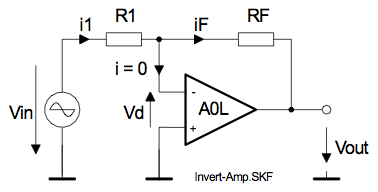
\includegraphics[width=6cm]{./bilder/i-verstaerker.png}
      \end{minipage}\\
      
		\subsubsection{Nichtinvertierender Verstärker}
			Beim nichtinvertierenden Verstärker ist die Ausgangsspannung
      gleichphasig zur Eingangsspannung.\\ 
			\begin{minipage}[T]{12cm}
      	
        \begin{tabular}{ll}
        	Closed-Loop Gain: &
        	$A_{CL}=\frac{v_{out}}{v_{in}}=\frac{R_F}{R_1}+1$\\
        	& $v_{out} = v_{in}\cdot(\frac{R_F}{R_1}+1)$ \\
        	$i_1=\frac{v_{in}-v_d}{R_1}$ &
        	$i_F=\frac{v_{out}}{R_F+R_1}$\\
          Ausgangswiderstand des NI-Verstärkers: &
          $r_{out}=0\Omega$\\
          Eingangswiderstand des NI-Verstärkers: &
          $r_{in}=\infty$\\
        \end{tabular}
      \end{minipage}
			\begin{minipage}{6cm}
      	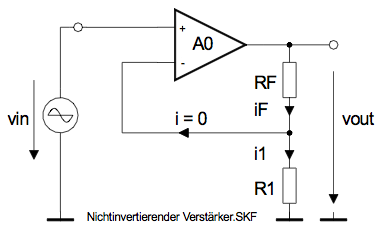
\includegraphics[width=6cm]{./bilder/ni-verstaerker.png}
      \end{minipage}\\

		\subsubsection{Verstärker mit mehreren Eingängen}
			\begin{minipage}{12.5cm}
            	$A_{CL1}=-\frac{R_F}{R_1}$\\
            	$A_{CL2}=-\frac{R_F}{R_2}$\\
            	$A_{CL3}=\frac{R_F+(R_1//R_2)}{(R_1//R_2)}$\\
            	$v_{out}=A_{CL1}v_1+A_{CL2}v_2+A_{CL3}v_3=
            	-\frac{R_F}{R_1}v_1-\frac{R_F}{R_2}v_2+\frac{R_F+(R_1//R_2)}{(R_1//R_2)}$\\
      \end{minipage}
			\begin{minipage}{5.5cm}
      	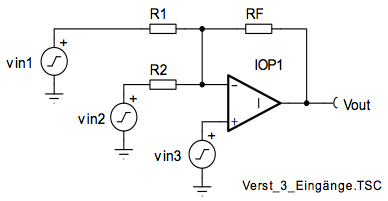
\includegraphics[width=5.5cm]{./bilder/3-eingaenge.png}
      \end{minipage}\\

		\subsubsection{Invertierender Addierer}
			\begin{minipage}[b]{12cm}
            $V_{out}=A_{CL1}V_{IN1}+A_{CL2}V_{IN2}+\ldots$\\
            $V_{out}=- \frac{R_F}{R_1}V_{IN1}- \frac{R_F}{R_2}V_{IN2}+\ldots$\\
            $A_{CL1}=- \frac{R_F}{R_1}$\\
           	$A_{CL2}=- \frac{R_F}{R_2}$\\
      \end{minipage}
			\begin{minipage}{6cm}
      	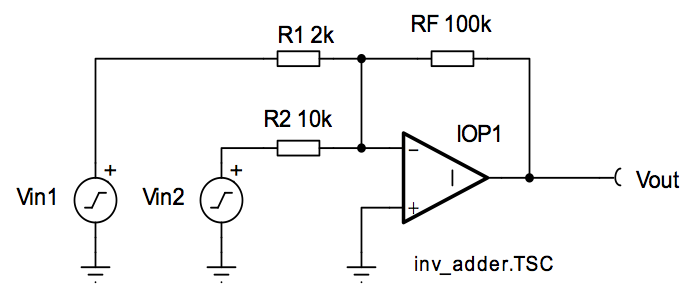
\includegraphics[width=6cm]{./bilder/invertadd.png}
      \end{minipage}\\

		\subsubsection{Gewichteter Subtrahierer}
			\begin{minipage}[b]{12cm}
            	$A_{CL1}=- \frac{R_F}{R_1}$\\
            	$A_{CL2}=
           		\frac{R_3}{R_3+R_2}\left(1+\frac{R_F}{R_1}\right)$\\
            	$v_{out}=
            	\frac{R_3}{R_3+R_2}\left(1+\frac{R_F}{R_1}\right)
            	v_{in2}-\frac{R_F}{R_1}v_{in1}$\\
      	\end{minipage}
			\begin{minipage}{6cm}
            	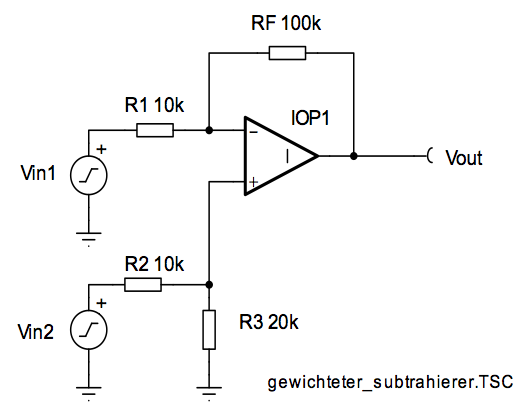
\includegraphics[width=6cm]{./bilder/gewichtsub.png}
            \end{minipage}\\


		\subsubsection{Mehrfach-Addierer-Subtrahierer} 		
		\begin{minipage}[b]{12cm}
		1. Man waehlt $R_{F}$\\
		2. Man waehlt $R_{P}$, wobei oft $R_{P}=R_{F}$ gesetzt wird. (optional)\\
		3. $R_{n}=\frac{R_{F}}{\left|A_{n}\right|}$ oder
			$R_{n}=\frac{R_{P}}{\left|A_{n}\right|}$\\ 
		4. Verstärkungsbedingung: $A_{N1} +
		\ldots + A_{Nn} = A_{P1} + \ldots + A_{Pn}$ \\Falls unerfüllt, muss ein Dummyeingang hinzugefügt werden!
		\end{minipage}
		\begin{minipage}{6cm}
          	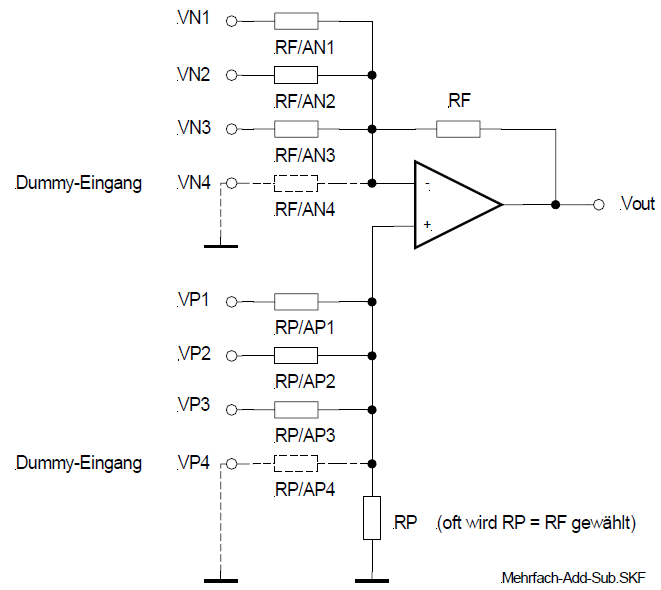
\includegraphics[width=6cm]{./bilder/mehrfach-addierer-subtrahierer.png} 
        \end{minipage}\\

		\subsubsection{Instrumentenverstärker}
		\begin{minipage}[b]{12cm}
		$A_{diff}=\frac{V_{out}}{V_{diff}}=\frac{V_{P}-V_{N}}{V_{inP}-V_{inN}}
		=\frac{2R_{1}+P}{P}=\frac{2R_{1}}{P}+1$\\
		\end{minipage}
		\begin{minipage}{6cm}
          	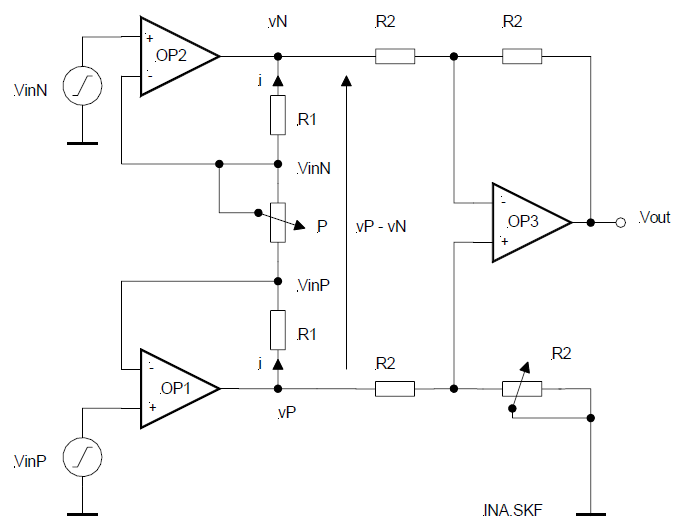
\includegraphics[width=6cm]{./bilder/Instrumentationsverstaerker.png} 
        \end{minipage}\\

		\subsubsection{Differenzverstärker}
			\begin{minipage}[b]{12cm}
            	$A_{diff}=\frac{v_{out}}{(v_{in2}-v_{in1})}$\\
            	$v_{out} = \frac{R_F}{R_1}\cdot (v_{in2}-v_{in1})$\\
            	Widerstandsbedingung für den Differenzverstärker\\
            	$A_{diff}=\frac{R_F}{R_1}=\frac{R_3}{R_2}$\\
            \end{minipage}
			\begin{minipage}{6cm}
            	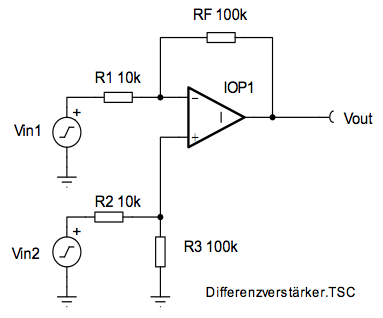
\includegraphics[width=6cm]{./bilder/differenzver.png}
            \end{minipage}\\


		\subsubsection{Komparatorschaltung}
			\begin{minipage}{18cm}
            	Wenn ein Operationsverstärker als {\it Verstärker ohne
            	Gegenkopplung} betrieben wird, spricht man von einer {\it
            	Komparatorschaltung}. Der Operationsverstärker wird dann als {\it
            	Komparator} betrieben.\\
            	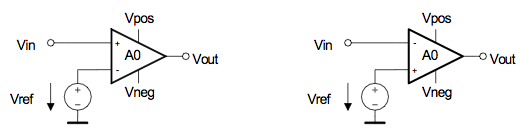
\includegraphics[width=16cm]{./bilder/komparator.png}\\
            	Beim nichtinvertierenden Komparator (links)\\
            	$V_{out}=V_{out\hspace{1mm}max}=V_{pos}-V_{Rand}
            	\mbox{ wenn } V_{in} > V_{ref}\pm V_{OS} \mbox{ bzw. } 
            	V_{diff}\pm V_{OS}>0$\\
            	$V_{out}=V_{out\hspace{1mm}min}=V_{neg}+V_{Rand}
            	\mbox{ wenn } V_{in} < V_{ref}\pm V_{OS} \mbox{ bzw. } 
            	V_{diff}\pm V_{OS}<0$\\ \\
            	Beim invertierenden Komparator (rechts)\\
            	$V_{out}=V_{out\hspace{1mm}max}=V_{pos}-V_{Rand}
            	\mbox{ wenn } V_{in} < V_{ref}\pm V_{OS} \mbox{ bzw. } 
            	V_{diff}\pm V_{OS}<0$\\
            	$V_{out}=V_{out\hspace{1mm}min}=V_{neg}+V_{Rand}
            	\mbox{ wenn } V_{in} > V_{ref}\pm V_{OS} \mbox{ bzw. } 
            	V_{diff}\pm V_{OS}>0$\\
            \end{minipage}

		\subsubsection{Schmitt-Trigger}
		Nichtinvertierender Schmitt-Trigger\\
			\begin{minipage}{9cm}
	          	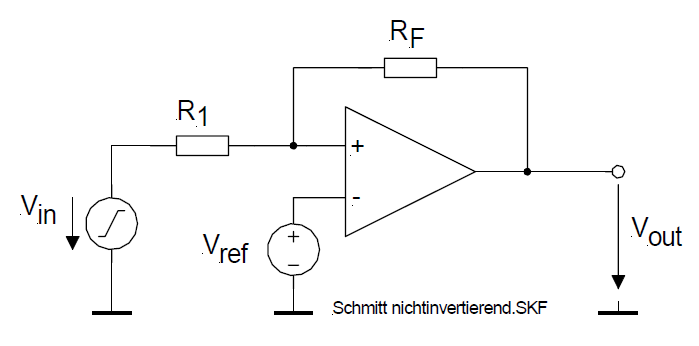
\includegraphics[width=8cm]{./bilder/n-schmitt.png} 
	        \end{minipage}
			\begin{minipage}{9cm}
	          	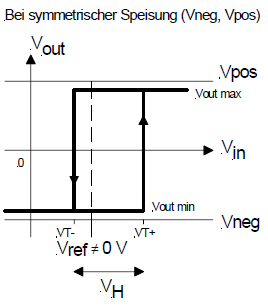
\includegraphics[width=4cm]{./bilder/n-schmitt-kennlinie.png} 
	        \end{minipage}\\
		Invertierender Schmitt-Trigger\\
			\begin{minipage}{9cm}
	          	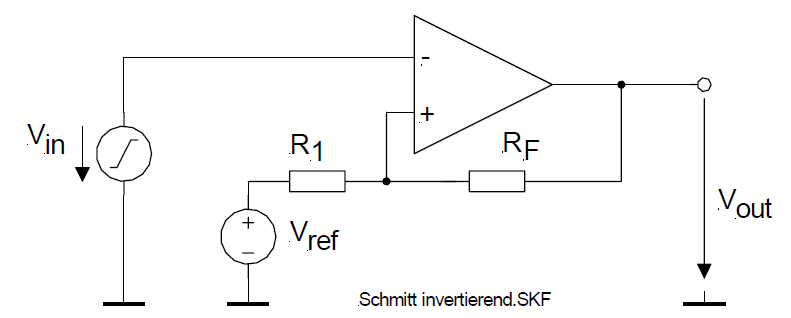
\includegraphics[width=8cm]{./bilder/i-schmitt.png} 
	        \end{minipage}
			\begin{minipage}{9cm}
	          	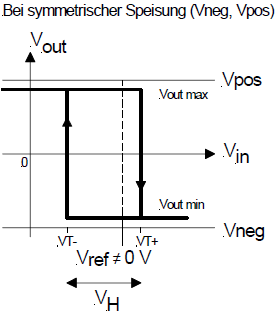
\includegraphics[width=4cm]{./bilder/i-schmitt-kennlinie.png} 
	        \end{minipage}\\
			
			\begin{minipage}{18cm}
               	Hysteresespannung:\\
               	\hspace*{10mm}
               	\begin{tabular}{| c | c |}
                \hline
                Nichtinvertierender Schmitt-Trigger & Invertierender
                Schmitt-Trigger\\
                \hline
                $V_H=(V_{out \hspace{1mm} max}-V_{out \hspace{1mm}
                min})\frac{R_1}{R_F}$ &
                $V_H=(V_{out \hspace{1mm} max}-V_{out \hspace{1mm}
                min})\frac{R_1}{R_1+R_F}$\\
                \hline
            \end{tabular}\\ \\
				Schwellspannung:\\
				\hspace*{10mm}
			\begin{tabular}{| c | c |}
                \hline
                Nichtinvertierender Schmitt-Trigger & Invertierender
                Schmitt-Trigger\\
                \hline
                $V_{T+}=V_{ref}+(V_{ref}-V_{out
                \hspace{1mm} min})\frac{R_1}{R_F}$ &
                $V_{T+}=V_{ref}+(V_{out \hspace{1mm}
                max}-V_{ref})\frac{R_1}{R_1+R_F}$\\
                \hline
                $V_{T-}=V_{ref}-(V_{out
                \hspace{1mm} max}-V_{ref})\frac{R_1}{R_F}$ &
                $V_{T-}=V_{ref}-(V_{ref}-V_{out \hspace{1mm}
                min})\frac{R_1}{R_1+R_F}$\\
                \hline
            \end{tabular}\\
            \end{minipage}
	
		\subsubsection{Differentiator}
			\begin{minipage}[b]{12cm}
           		Beim Differentiator gilt $v_{out}=v_N-i_1 \cdot R_F$ wobei
           		$v_N=0$\\
           		$i_1=C_1 \cdot \frac{dv_C}{dt}$\\
           		$v_{out}=-R_FC_1 \frac{dv_{in}}{dt}$\\
           		Die Elemente $C_F$ und $R_1$ sind optional. \\
           		Sie beheben jedoch Probleme die ohne \\
           		sie entstehen (siehe elemenarer Differentieator). \\
           		Mit $C_F$ und $R_1$: \\
           		- Keine differentiation bei hoeheren Frequenzen. \\
           		- Limitierte Verstaerkuing bei hoeheren Frequenzen. \\
           		- Eingangswiderstand immer groesser $R_1$ \\ 
           		$\rightarrow$ keine Belastung der Signalquelle
           
           	\end{minipage}
			\begin{minipage}{6cm}
           		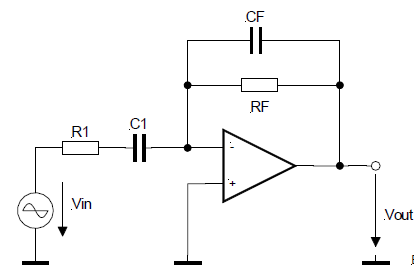
\includegraphics[width=6cm]{./bilder/differentiator.png}
           	\end{minipage}

		\subsubsection{Integrator} 
		\vspace{1cm}
		\begin{minipage}[b]{12cm}
		$v_{out}=-\frac{1}{RC} \int{v_{in}}dt +
		v_{out\hspace{1mm}Anfang} $\\
		$\frac{dv_{out}}{dt}=-\frac{v_{in}}{RC}$\\
		\end{minipage} 
		\begin{minipage}{6cm}
          	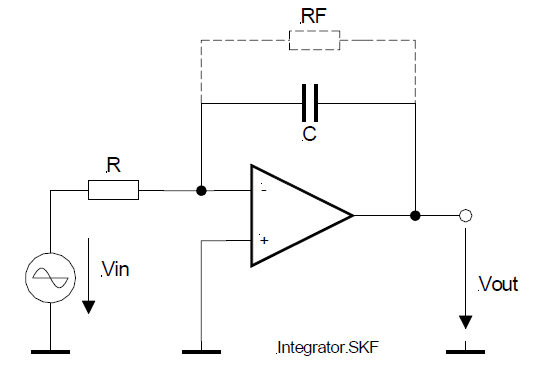
\includegraphics[width=6cm]{./bilder/integrator.png} 
        \end{minipage}\\

	\subsection{Fehlereinflüsse des Opamp}
		\subsubsection{Verstärkungsfehler bei endlicher Closed-Loop-Verstärkung}
			\begin{minipage}{12cm}
				\begin{tabular}{ll}
               	beim nichtinvertierenden Verstärker &
               	$A_{CL \hspace{1mm} ideal}=\frac{R_F}{R_1}+1$\\
               	beim invertierenden Verstärker &
                $A_{CL \hspace{1mm}
               	ideal}=-\frac{R_F}{R_1}$\\
         \end{tabular}
               	Beim invertierenden Verstärker ist eine kleine Korrektur
               	anzubringen: \\
               	$\frac{1}{A_{CL \hspace{1mm}
               	real}}=\frac{1}{A_{CL \hspace{1mm} real}}+\frac{1}{nA_{OL}}$\\
	        \end{minipage}
			\begin{minipage}{6cm}
               	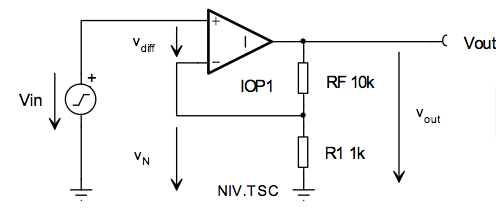
\includegraphics[width=6cm]{./bilder/verstaerkungsfaktor.png}
            \end{minipage}
		\subsubsection{Offsetspannungsfehler}
				\begin{tabular}{ll}
					Im Closed-Loop-Betrieb ist die Ausgangs-Fehlerspannung: &
					$V_{out \hspace{1mm}E}=V_{OS}\left( 1+\frac{R_F}{R_1}\right)$\\
          allgemein: &
          $V_{out \hspace{1mm}E}=V_{OS} \cdot {A_{CL}}^{+}$\\
          Im Open-Loop-Betrieb ist die Ausgangs-Fehlerspannung: &
          $V_{out \hspace{1mm}E}=V_{OS}\cdot {A_{CL}}^{+}$\\
         \end{tabular}
		
		\subsubsection{Eingangsstromfehler}
			\begin{minipage}{18cm}
              Wenn die Opamp-Eingangsströme gleich gross sind
              ($I_{N}=I_{P}$) und die Gleichstromwiderstände,
              die von jedem Opamp-Eingang nach Masse führen, 
              ebenfalls gleich gross gewählt werden, heben sich die
              Ausgangsspannungsfehler, die durch $I_{N}$ und $I_{P}$
              erzeugt werden, gegenseitig auf. \\
              \begin{tabular}{ll}
              Allgemeine Formel für den
              Eingangsstromfehler: &
              $V_{out \hspace{1mm}E}=I_N R_F-R_2 I_P\left( 1+\frac{R_F}{R_1} \right)$\\
              Widerstandsbedingung für Eingangsstromkompensation:&
              $R_2=\frac{R_F R_1}{R_F+R_1}=R_F // R_1$\\
            	\end{tabular}
            \end{minipage}\\
			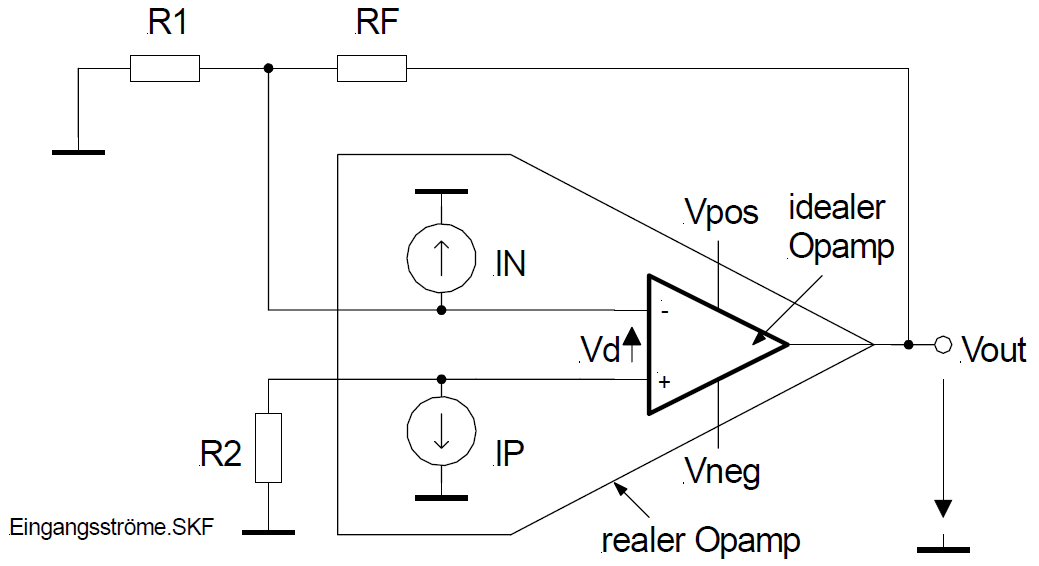
\includegraphics[width=8cm]{./bilder/eingangsstromfehler.png}

		\subsubsection{Eingangsstromkompensation ohne AC-Zweige}
			\begin{minipage}[b]{6cm}
            	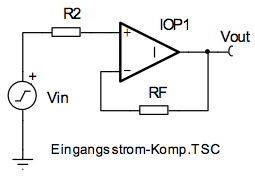
\includegraphics[height=3cm]{./bilder/spannungsfolger.png}\\
            	\centerline{{\bf Spannungsfolger}}\\ \\
            	$R_2$ sei ein gegebener Quellen-Widerstand\\
            	{\bf $R_F$ muss eingefügt werden}\\ \\
            	$R_F=R_2$
            \end{minipage}\hfill
			\begin{minipage}[b]{6cm}
            	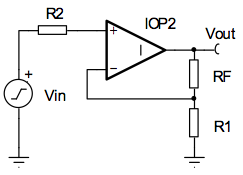
\includegraphics[height=3cm]{./bilder/nichtinver}\\
            	\centerline{{\bf Nichtinvertierender Verstärker}}\\ \\
            	Hier sei der Quellenwiderstand
            	vernachlässigbar.\\ {\bf $R_2$ muss eingefügt werden}\\ \\
            	$R_2=R_F//R_1$
            \end{minipage}\hfill
			\begin{minipage}[b]{6cm}
            	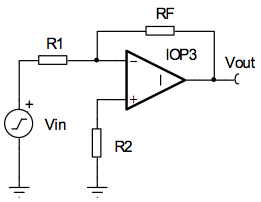
\includegraphics[height=3cm]{./bilder/inver}\\
            	\centerline{{\bf Invertierender Verstärker}}\\ \\ \\ \\
            	{\bf $R_2$ muss eingefügt werden}\\ \\
            	$R_2=R_F//R_1$
            \end{minipage}
			\begin{minipage}{18cm}
            	\vspace{3mm}
				\textbf{Ausgangsspannungsfehler} auf Grund des \textbf{Offsetstromes} (nur bei
				Kompensation(!)):
				\fbox{$V_{out \hspace{1mm}E}=\left|I_{OS}\right| \cdot R_F$}\\
			\end{minipage}

		\subsubsection{Zusammenfassung aller Fehlereinflüsse}
      $V_{out\hspace{1mm}E\hspace{1mm}total}=A_{CL+}\cdot\left[\left|V_{OS}\right|+\frac{\left|V_{CM}\right|}{CMRR}
            	+\frac{\left|\Delta V_{Supply}\right|}{PSRR}\right]+\left|I_{OS}\right|R_F$\\

	\subsection{Dynamische Eigenschaften des Opamp}
		\begin{tabular}{ll}
			dB-Verstärkung:&
			$A_{dB}=20 \cdot log A_{lin}$\\
			lineare Verstärkung:&
			$A_{lin}=10^{\frac{A_{dB}}{20}}$\\
		\end{tabular}
		Verstärkungs-Bandbreite-Produkt GBP (Gain-Bandwidth-Product)\\
		\begin{tabular}{ll}
			Bandbreite des gegengekoppelten {\it nichtinvertierenden} Verstärkers:&
			$f_{CL+}=\frac{GBP}{A_{CL \hspace{1mm}lin}}$\\
			Bandbreite des gegengekoppelten {\it invertierenden} Verstärkers: &
			$f_{CL}=\frac{GBP}{\left| A_{CL \hspace{1mm}lin}\right|+1}$\\
		\end{tabular}\\
		{\bf Gesetz vom Konstanten Verstärkungs-Bandbreite-Produkt:} \\
		Für jeden Punkt auf der mit -20dB abfallenden Frequenzgang-Gerade ist das
		Produkt aus Verstärkung und zugehöriger Frequenz konstant gleich GBP, d.h. $A_{lin}\cdot f=GBP=konst$\\
		\subsubsection{Slew-Rate}
			\begin{tabular}{ll}
				min. SR bei einem Sprungsignal &
				$SR\geq\frac{0.8V_{step}}{t_{anstieg}}$\\ 
				min. SR bei einem Sinussignal & 
				$SR\geq V_{amplitude}\omega=V_{amplitude}2\pi f$\\
			\end{tabular}

			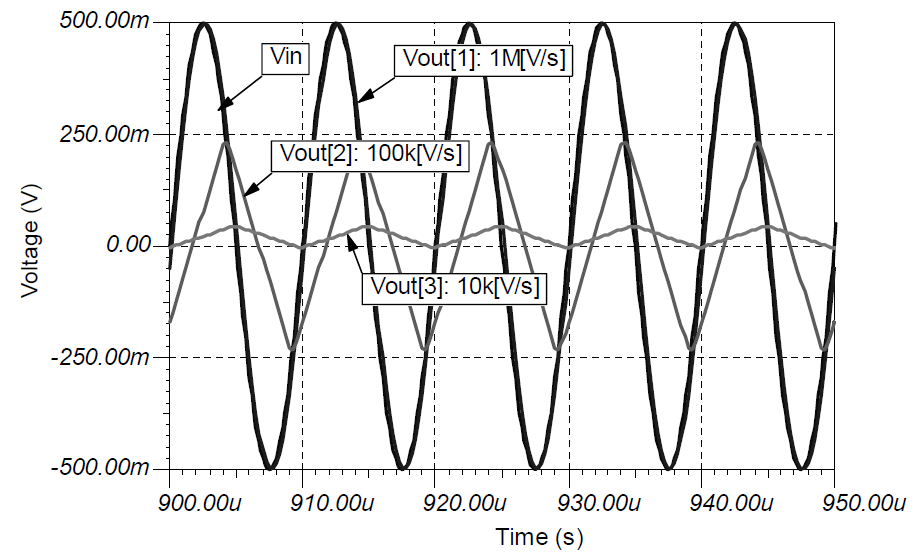
\includegraphics[height=5cm]{./bilder/slew-rate.png}\\

			{\bf Anstiegszeit des Ausgangs:} \\
			\begin{tabular}{ll}
				$t_{rout}$ & = $\sqrt{t_{rin}^2 + t_{rAmp}^2}$ \\
				$t_{rin}$  & = Anstiegszeit des Eingangssignals \\
				$t_{rout}$ & = Anstiegszeit des Ausgangssignals \\
				$t_{rAmp}$ & = $\frac{0.35}{f_{bw}} = $ Eigenanstiegszeit des Verstärkers \\
				$f_{bw}$   & = Kleinsignalbandbreite des Verstärkers \\
			\end{tabular}


\newpage
\section{Grundlagen Halbleiter}
	\begin{minipage}{8cm}
		\begin{align*}
			R &= \frac{\rho \cdot l}{A} = \frac{l}{\kappa \cdot A} \\
			\kappa &= \frac{1}{\rho}  = n \cdot q \cdot \mu \\
			\kappa &= n_i \cdot q \cdot \left( \mu_n - \mu_p \right) \\
			n_i^2 &= n_0 \cdot p_0 \\
			\rho(T) &= \rho(T_0) \cdot \left(1 + \alpha(T-T_0)\right)
		\end{align*}
	\end{minipage}
	\begin{minipage}{8cm}
		\begin{tabular}{lll}
		$\kappa$	& $[{m}/{\Omega mm^2}]$	& spezifische Leitfähigkeit \\
		$\rho$		& $[{\Omega mm^2}/{m}]$	& spezifischer Widerstand \\
		$n$			& $[cm^{-3}]$ & Ladungsträgerdichte \\
		$n_i$		& $[cm^{-3}]$ & Eigenleitungsdichte \\
		$n_0$		& $[cm^{-3}]$ & Elektronendichte \\
		$p_0$		& $[cm^{-3}]$ & Löcher-Dichte \\
		$q$			& $[As]$	& Elementarladung $q=1,6 \cdot 10^{-19} As$ \\ 
		$\mu$		& $[{cm^2}/{Vs}]$	& Beweglichkeit der Ladungsträger \\
		$l$			& $[m]$	& Länge \\
		$A$			& $[mm^2]$	& Fläche \\
		$\alpha$	& $[K^{-1}]$ & Temperaturkoeffizient \\
		$T$			& $[K]$	& Temperatur \\
		\end{tabular}
	\end{minipage}
\section{Dioden}
	Sperrstromdichte v. Si-Dioden: $10^{-11} \frac{A}{cm^2}$ \\
	\begin{tabular}{l l}
			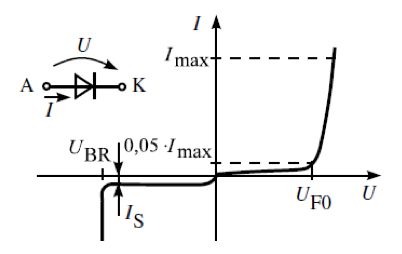
\includegraphics[width=6cm]{./images/Diode-Kennlinie.png}
		&	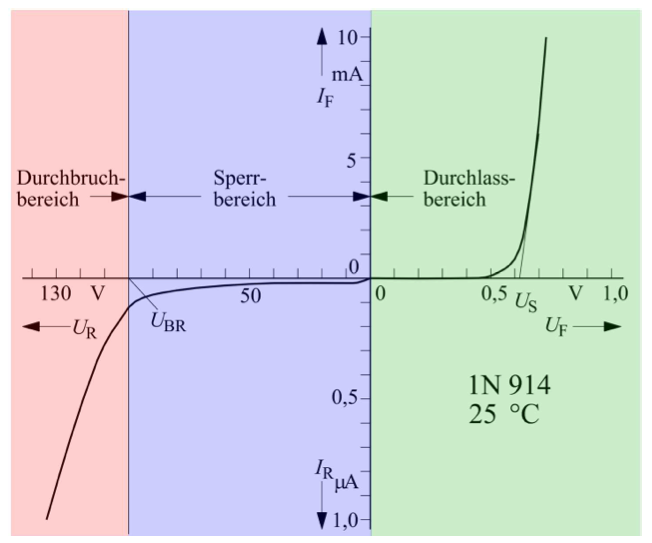
\includegraphics[width=6cm]{./images/Diode-Kennlinie-2.png}
	\end{tabular}
	
	\subsection{Kleinsignal-ESB}
		\begin{tabular}{l l}
			\multirow{5}{*}{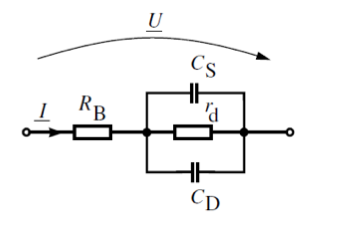
\includegraphics[width=4cm]{./images/Diode-KS-ESB.png}}
			& $R_B$: Bahnwiderstand (inkl. Zuleitung, Kontaktierung) \\
			& $r_d$: differentieller Widerstand des pn-Übergangs \\
			& $C_D$: Diffusionskapazität (bei pos. Diodenspannung) \\
			& $C_S$: Sperrschichtkapazität (bei neg. Diodenspannung)\\
			& $r_d=\frac{dU}{dI}$ (Tangentensteigung im AP) \\
		\end{tabular}
	
	\subsection{Grosssignal-ESB}
		\begin{tabular}{l l}
			\multirow{6}{*}{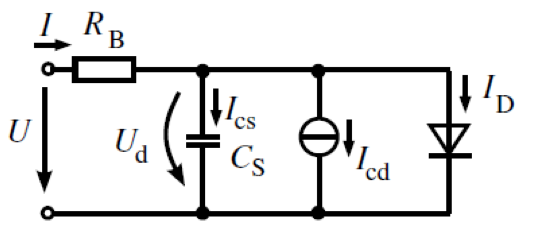
\includegraphics[width=4cm]{./images/Diode-GS-ESB.png}}
			& Gleichstromwiderstand $R_D = \frac{U_0}{I_0}$ (im AP)\\
			& $I=I_S \cdot (e^{\frac{U}{m \cdot U_T}}-1)$ \\
			& $I_S$: Sättigungssperrstrom (Bereich: $pA$)\\
			& $m$: Emissionskoeffizient (meistens: $m=1$) \\
			& $U_T=\frac{kT}{q} \approx 26mV$ \\
			& beim Umschalten bewirken die Kapazitäten $C_S$ und $C_D$ eine Verzögerung \\
		\end{tabular}
		
	\subsection{Temperaturverhalten}
		Faustregel: Durchflusspannung $U_{F0}$ ändert um $-2 \frac{mV}{K}$! Der Sperrstrom verdoppelt sich je Temperaturunterschied à $10K$ \\
		
		\textbf{Thermospannung $U_T$:} \\
		\begin{minipage}{6cm}
			\begin{align*}
				U_T &= \frac{k_B \cdot T}{q} \\
				U_{T_{23^{\circ}C}} &= 25,5 mV 
			\end{align*}
		\end{minipage}
		\begin{minipage}{10cm}
			\begin{align*}
			k_B &= 1,38065 \cdot 10^{-23} J/K &\text{Boltzmann-Konstante} \\
			q &= 1,60218 \cdot 10^{-19} As &\text{Elementarladung} \\
			\end{align*}
		\end{minipage}

	
\newpage	
	\subsection{Spezielle Dioden und Anwendungen}
		\subsubsection{Gleichrichter-Diode}
			\begin{minipage}[T]{6cm}
				\textbf{Einweg-Gleichrichter} \\
				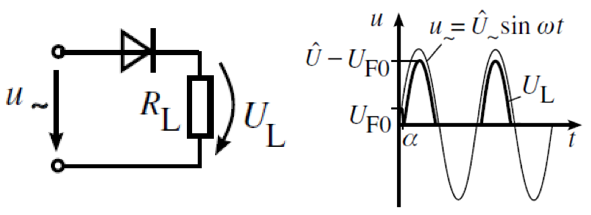
\includegraphics[width=5cm]{./images/gleichrichter-einweg} \\
			\end{minipage}
			\begin{minipage}[T]{6cm}
				\textbf{Gleichrichter mit Glättung} \\
				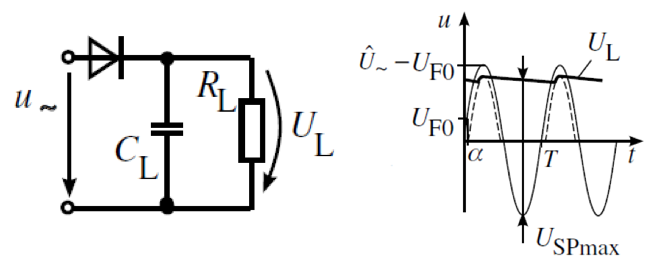
\includegraphics[width=5cm]{./images/gleichrichter-einweg-glaettung} \\
				Bedingung: $\tau = R_L \cdot C_L \gg T$ \\
			\end{minipage}
			\begin{minipage}[T]{6cm}
				\textbf{Brücken-Gleichrichter} \\
				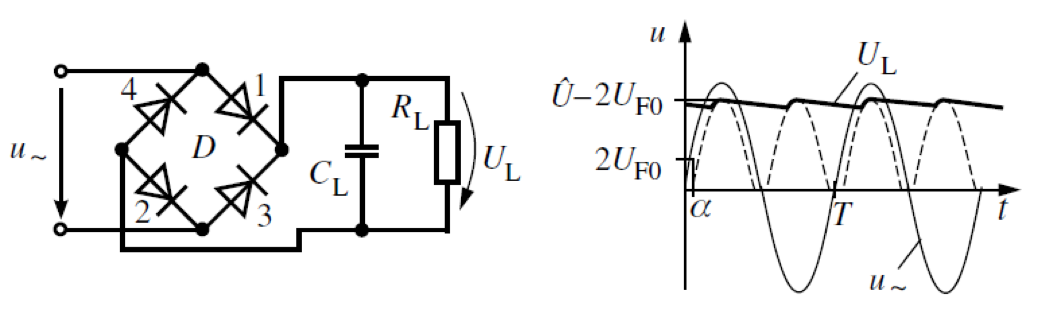
\includegraphics[width=6cm]{./images/gleichrichter-bruecke} \\
			\end{minipage}						

		\subsubsection{PIN-Diode}
			Für höhere Spannungsfestigkeit wird eigenleitende Halbleiterzone, die sog. 
			Intrinsic-Zone zwischen p- und n-dotierte Zone gelegt. Die Intrinsic-Zone
			ist im Sperrbetrieb sehr hochohmig und reduziert somit die el. Feldstärke
			auf ein akzeptables Mass.
		
		\subsubsection{Kapazitätsdiode}
			Kapazitätsdioden (Varicaps) werden in Sperrichtung betrieben. Die 
			Kapazität hängt dabei von der Spannung $U_{SP}$ ab.
			Anwendung: Einstellen der Schwingfrequenz in Oszillatoren \\
			
		\subsubsection{Tunneldiode}
			Tunneldioden besitzen eine sehr hohe Störstellenkonzentration und einen
			steilen Dotierungsverlauf. 
			
		\subsubsection{Zener-Diode}
			\begin{minipage}{6.5cm}
				\textbf{Kennline} \\
				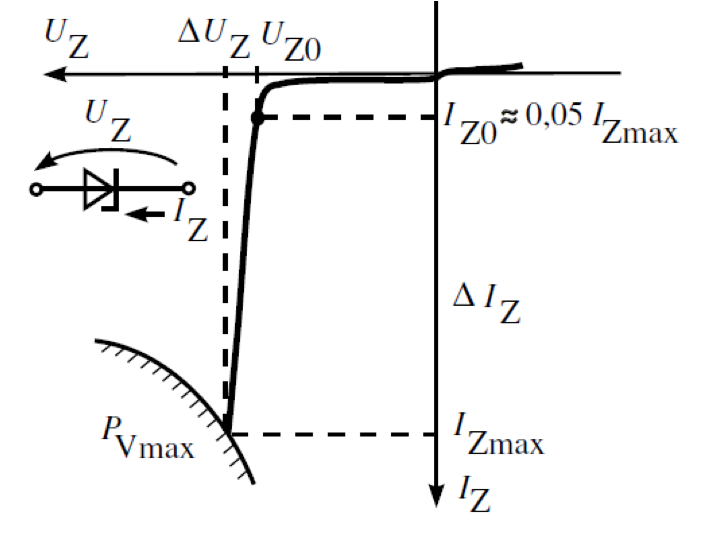
\includegraphics[width=6cm]{./images/zdiode-kennlinie.png}
			\end{minipage}
			\begin{minipage}{4.5cm}
				\textbf{Grosssignal-ESB:} \\
				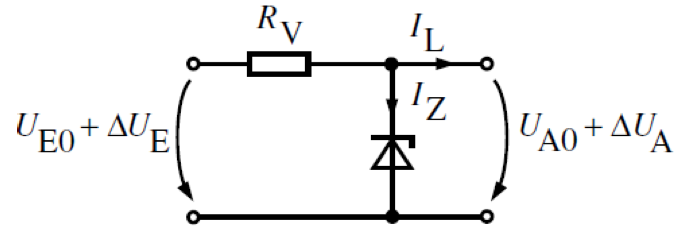
\includegraphics[width=4cm]{./images/zener-gs} \\
				\textbf{Kleinsignal-ESB:} \\
				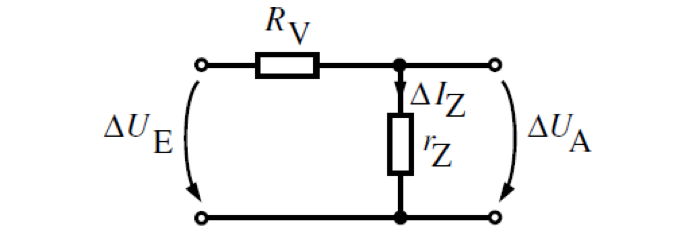
\includegraphics[width=4cm]{./images/zener-ks}
			\end{minipage}
			\begin{minipage}{7.5cm}
				Anstieg der Durchbruchkennlinie bei spezieller Dotierung. Anwendung: Spannungsbegrenzung und -stabilisierung  \\
				
				Temperaturkoeffizient abhängig von Zenerspannung. $~0$ bei $5.6V$ -
				darüber: negativer Temperaturkoeffizient\\
			\end{minipage} \\
			
		\subsubsection{Schottky-Diode}
			Anstatt der p-Zone hat die Schottky-Diode eine Metall-Zone. Weil vom Metall
			keine Löcher in den Halbleiter diffundieren, gibt es keine Diffusionskapazität
			und die Diode bekommt ein sehr schnelles Schaltverhalten und eine kleine
			Durchflussspannung $U_{F0} \approx 0,3V$. \\
			
		\subsubsection{Leuchtdiode}
			Leuchtdioden werden aus verschiedenen Substraten (Halbleitern) hergestellt,
			z.B. GaAs (Gallium-Arsenid), InGaN (Indium-Gallium-Nitrid) um verschiedene
			Farben (Wellenlängen) zu produzieren. Typisch sind: \\
			\begin{tabular}{|l|l|l|c|} \hline
				infrarot & $900nm$ & GaAs & $1,0-1,5V$ \\ \hline
				rot & $635nm$ & GaAsP & $1,6-2.2V$ \\ \hline
				grün & $565nm$ & GaP & $2,0-2,4V$ \\ \hline
				blau & $490nm$ & InGaN & $3,2-4,0V$ \\ \hline
			\end{tabular}\\
			
		\subsubsection{Photodiode}
			Photodioden werden in Sperr-Richtung angeschlossen. Der Sperrstrom erhöht sich
			bei Lichteinfall. Meistens werden Photodioden mit einen OP-Verstärker (als
			Transimpedanzverstärker) benutzt. \\
\section{Transitoren}
	\subsection{Transistortypen}
	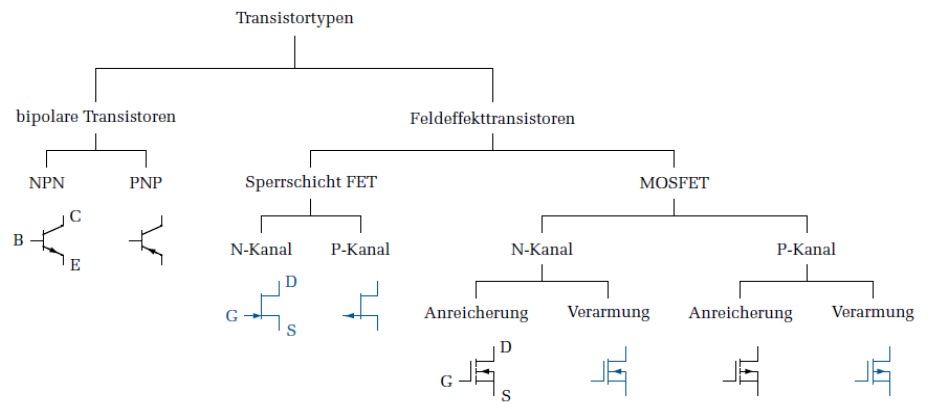
\includegraphics[width=11cm]{images/Transistortypen.png}

\subsection{Bipolartransistoren}
	\begin{minipage}[c]{6cm}
		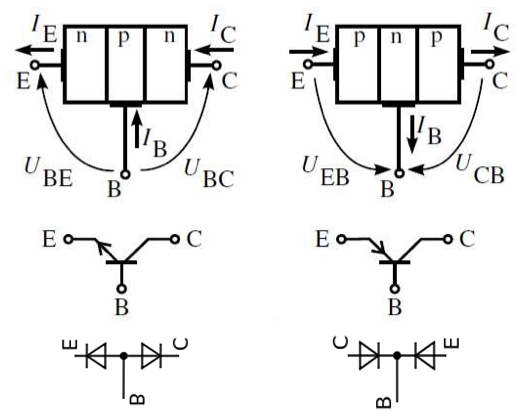
\includegraphics[width=6cm]{images/bipolarTransistor-Aufbau}
	\end{minipage}
	\begin{minipage}[c]{12cm}
		Links: NPN-Transistor \\
		Rechts: PNP-Transistor \\
		\\
		Die Schichten sind ungleich dick (Basis sehr dünn) und unterschiedlich dotiert.
		Sobald die BE-Diode Leitet, werden Elektronen vom Kollektor zur Basis gezogen und
		fliessen dann weiter zum Emitter. So steuert der Basisstrom $I_B$ den 
		Kollektorstrom $I_C$. \\
	\end{minipage} \\
	
	\begin{multicols}{2}
	\subsubsection{Betriebszustände}
		\begin{tabular}{l l}
			Normalbetrieb (Verstärker) & $V_{BE} > 0$, $V_{BC} < 0$\\
			Sättigung (Schalter EIN) & $V_{BE} > 0$, $V_{BC} > 0$\\
			Sperrbetrieb (Schalter AUS) & $V_{BE} < 0$, $V_{BC} < 0$\\
			Inversbetrieb (k. Anwendung) & $V_{BE} < 0$, $V_{BC} > 0$
		\end{tabular} \\
	\columnbreak
	\subsubsection{Stromverstärkungs-Faktoren}
		\begin{minipage}[c]{2.8cm}
			Basisschaltung \\
			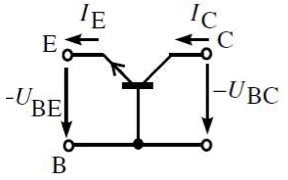
\includegraphics[width=2.8cm]{images/bip-basissch}\\
			$A_N=\frac{I_C}{I_E}$ \\
		\end{minipage}
		\begin{minipage}[c]{2.8cm}
			Emitterschaltung
			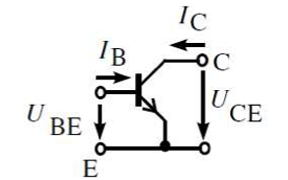
\includegraphics[width=2.8cm]{images/bip-emittersch}\\
			$B_N=\frac{I_C}{I_B}=\frac{A_N}{1-A_N}$ \\
		\end{minipage}
		\begin{minipage}[c]{2.8cm}
			Kollektorschaltung
			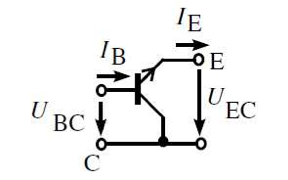
\includegraphics[width=2.8cm]{images/bip-kollektorsch}\\
			$C_N=\frac{I_E}{I_B}=\frac{1}{1-A_N}$ \\
		\end{minipage}
	\end{multicols}
	\subsubsection{Ebers-Moll-Modell}
		\begin{minipage}[c]{4cm}
			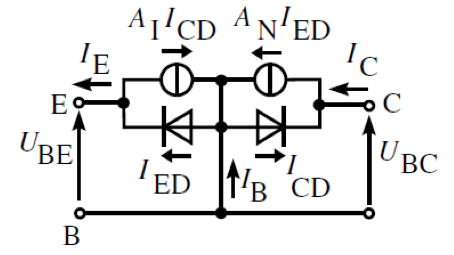
\includegraphics[width=4cm]{images/bipolar-EbersMoll}
		\end{minipage}
		\begin{minipage}[c]{8cm}
			$I_C=A_NI_{E_{sat}}(e^{\frac{U_{BE}}{U_T}}-1)
			 -I_{C_{sat}}(e^{\frac{U_{BC}}{U_T}}-1)$ \\
			$I_E=I_{E_{sat}}(e^{\frac{U_{BE}}{U_T}}-1)
			 -A_II_{C_{sat}}(e^{\frac{U_{BC}}{U_T}}-1)$ \\
			$I_B=I_E-I_C$ \\
		\end{minipage}
	
	\subsubsection{Kennlinien \& Formeln}
		\begin{minipage}[c]{4cm}
			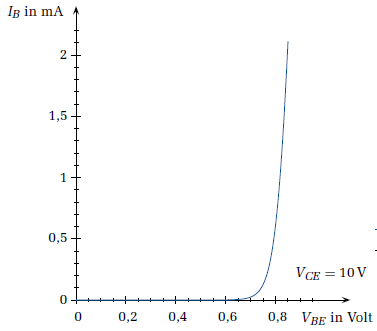
\includegraphics[width=4cm]{images/bipolarEingangsKennlinie}
		\end{minipage}
		\begin{minipage}[c]{5cm}
			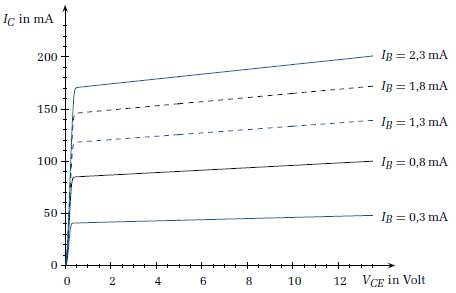
\includegraphics[width=5cm]{images/bipolarAusgangsKennlinie}\\
		\end{minipage}
		\begin{minipage}[c]{8cm}
			links: Eingangskennlinie - rechts: Ausgangskennlinie \\
			\\
			Kleinsignal-Widerstand: $r_{BE} = \frac{\delta V_{BE}}{\delta I_B} $ \\
			Basisstrom: $I_B=I_{B_{sat}}(e^{\frac{U_{BE}}{U_T}}-1)
						\approx I_{B_{sat}} e^{\frac{U_{BE}}{U_T}}$ \\
			Kollektorstrom: $I_C = B_N I_B+I_{CE_{0}} \approx B_N I_B$ \\
			
		\end{minipage}
	
	\subsubsection{Early-Effekt}
		\begin{minipage}[c]{5cm}
			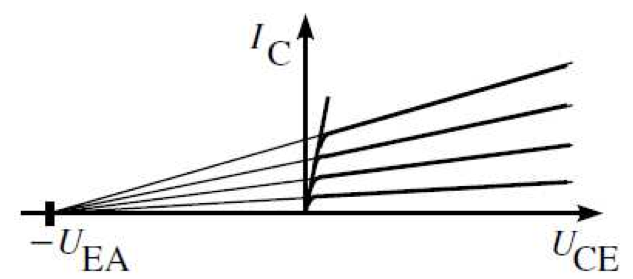
\includegraphics[width=5cm]{images/early-effekt}
		\end{minipage}
		\begin{minipage}[c]{12cm}
			Anstieg der Ausgangskennlinien beruht auf Veränderung der Basisweite infolge
			der Spannungsabhängigkeit der Sperrschichtweite der Basis-Kollektor-Diode. \\
			$U_{EA}$: Early-Spannung, Schnittpunkt der Ausgangskurven \\
			\\
			Modellerweiterung zur Berücksichtigung des Early-Effekts: \\
			$I_C = (B_NI_B+I_{CE_0})(1+\frac{U_{CE}}{U_{EA}}$
		\end{minipage}
		
	\subsubsection{Temperaturverhalten}
		Die maximale Leistung $P_V$ des Transistors muss stets kleiner als 
		$U_{CE} \cdot I_C$ sein. (Näherung) \\
		Zusätzlich muss die Wärme auch über das Gehäuse abgeführt werden können. Deshalb
		darf $P_V$ maximal $\frac{T_{max}-T_{amb}}{R_{th}}$ sein. ($R_{th}$: Thermischer
		Widerstand des Gehäuse) \\
		Der Transistor hat grundsätzlich das gleiche Temperaturverhalten wie die Diode. Somit
		gilt auch hier: $V_{BE}$ ändert um $-2\frac{mV}{K}$. Somit gilt für den
		Stromverstärkungsfaktor: $B_N=B_N(T_0)\cdot e^{C_b(T-T_0}$ mit 
		$C_b \approx 0.6\% \cdot K^{-1}$. Der hohe Temperatureinfluss muss bei der
		Schaltungsentwicklung berücksichtigt werden. \\
		
	\subsection{Kleinsignalverhalten}
		Beim Kleinsignal-Ersatzschaltbild wird das Verhalten des Transistors im Arbeitspunkt
		approximiert . Dazu wird ein Arbeitspunkt $AP$ im Kennlinienfeld eingezeichnet
		und dort linearisiert. \\
		\begin{minipage}[c]{6cm}
			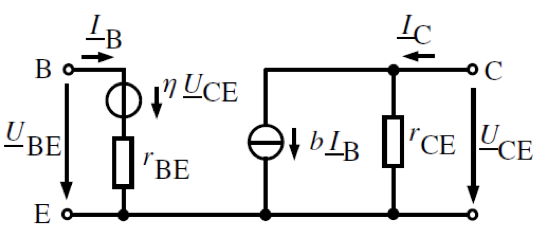
\includegraphics[width=6cm]{images/bip-kleinsignal}
		\end{minipage}
		\begin{minipage}[c]{6cm}
			$h_{11e} = r_{BE} = \frac{dU_{BE}}{dI_{B}} = \frac{U_T}{I_{B_0}}$ \\
			$h_{12e} = \eta = \frac{dU_{BE}}{dU_{CE}} \approx 0$ \\
			$h_{21e} = b = \frac{dI_C}{dI_B} = B_N(1+\frac{U_{CE_0}}{U_{EA}}) \approx B_N$ \\
			$h_{22e} = \frac{1}{r_{CE}} = \frac{dI_C}{dU_{CE}} = \frac{U_{EA}}{I_{C0}}$ \\
			$S = \frac{b}{r_{BE}}$
		\end{minipage}
		\begin{minipage}[c]{6cm}
			$r_{BE}$: Kleinsignal-Eingangswiderstand \\
			$\eta$: Kleinsignal-Spannungsrückwirkung \\
			$b$: Kleinsignal-Stromverstärkung \\
			$r_{CE}$: Kleinsignal-Ausgangswiderstand \\
			$S$: Kleinsignal-Steilheit
		\end{minipage} \\
		Kleinsignalmodell ohne Rückwirkung: $\eta \cdot U_{CE}$ wird weggelassen, weil 
		$\eta \approx 0$. Somit gilt: \\
		\begin{center}
			$\boxed{U_{BE} = r_{BE} \cdot I_B}$ \hspace{1cm} und \hspace{1cm}
			$\boxed{I_C = b \cdot I_B + \frac{1}{r_{CE}} \cdot U_{CE}}$ \\
		\end{center}
		
		Somit gilt für die \textbf{Emitterschaltung}: \\
		\begin{minipage}[c]{6cm}
			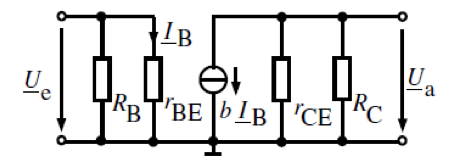
\includegraphics[width=6cm]{images/emittersch-esb}
		\end{minipage}
		\begin{minipage}[c]{12cm}
			$U_a = -b \cdot I_B \cdot (R_C || r_{CE})$ und $I_B=\frac{U_e}{r_{BE}}$ \\
			somit: $V_u = \frac{U_a}{U_e} = -\frac{b(R_C || r_{CE}}{r_{BE}}$ 
		\end{minipage} \\
		
	\subsection{Transistor als Schalter}
		
\subsection{Feldeffekt-Transistoren}

            \subsubsection{JFET Junction Field Effect Transistor}
            \begin{minipage}[T]{8cm}
                JFET als {\bf Konstantstromquelle}:\\
                benötigter Strom \fbox{$I_D = \frac{U_{GS}}{R_S}$}\\
                $U_{GS}$ entsprechend benötigem Strom aus Kennlinie lesen\\
                bei der Pinch-off-Grenze (Abschnürgrenze) sperrt der JFET
            \end{minipage}
            \begin{minipage}[T]{3.4cm}
                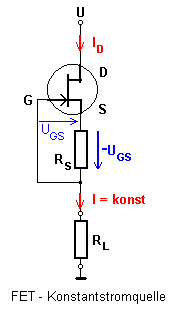
\includegraphics[height=4cm]{./images/JFETCCQuelle.png}
            \end{minipage}
            \begin{minipage}[T]{6cm}
                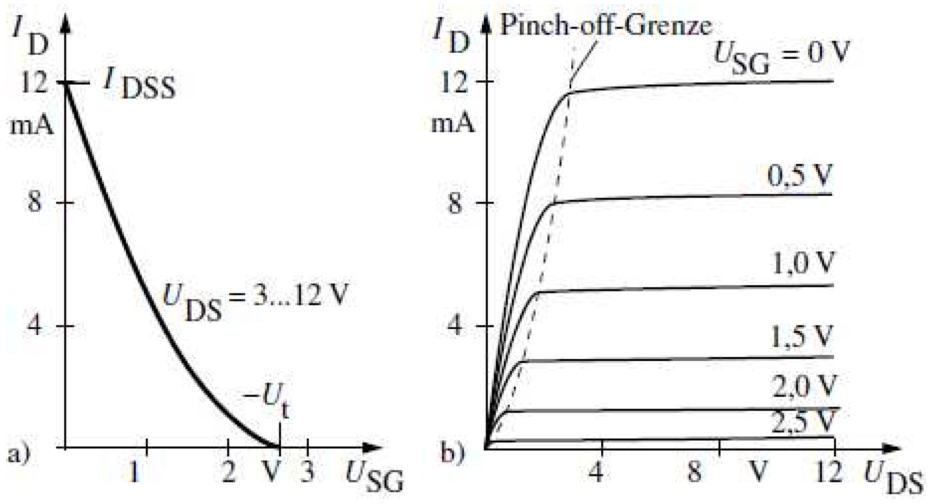
\includegraphics[height=4cm]{./images/JFETKennlinie.png}
            \end{minipage}
\hrule
            \subsubsection{MOSFET Metal Oxide Silicon Field Effect Transistor}
            \begin{minipage}[T]{6cm}
                \underline{Sperrbereich}\\\\
                $V_{GS} < V_{th} \to I_D = 0$\\
                typische $V_{th} = 0.5 \dots 1.5V$\\ 
                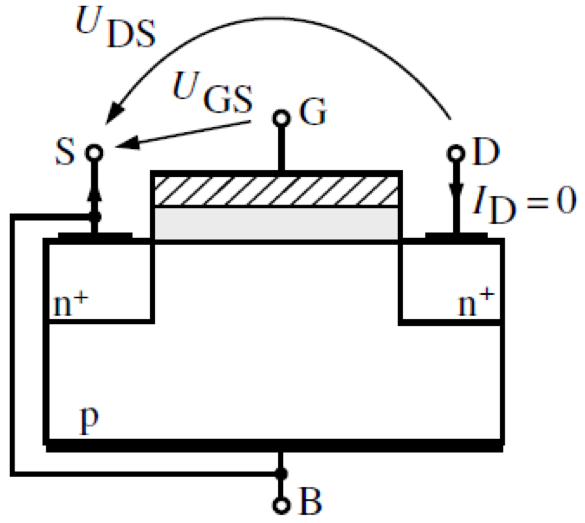
\includegraphics[height=4cm]{./images/MOSFETSperrbereich.png}
            \end{minipage}
            \begin{minipage}[T]{6cm}
                \underline{Widerstands-/Triodenbereich (linear)}\\\\
                $V_{GS} > V_{th} $ und $V_{DS}>0$\\
                $\to I_D$ fliesst\\
                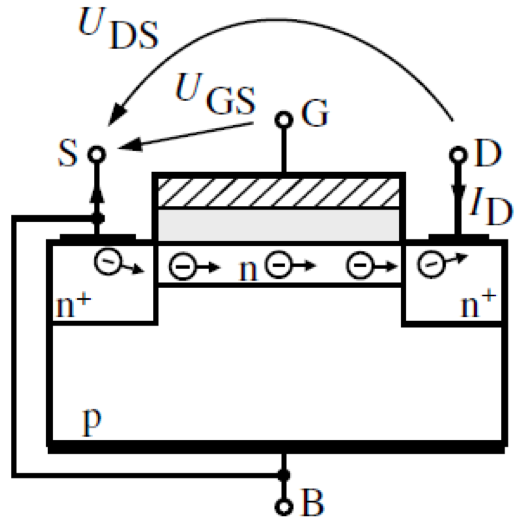
\includegraphics[height=4cm]{./images/MOSFETLinBereich.png}
            \end{minipage}
            \begin{minipage}[T]{6cm}
                \underline{S\"attigungs-/Pentodenbereich}\\\\
                $V_{DS} > V_{GS} - V_{th}$ Kanal wird abgeschnürt\\
                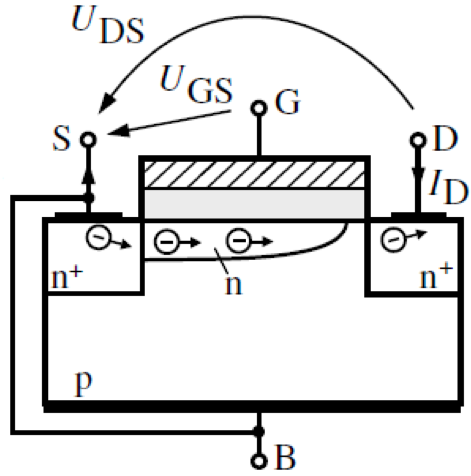
\includegraphics[height=4cm]{./images/MOSFETSaettBereich.png}
            \end{minipage}\\
            
            \subsubsection{Steuerkennlinien von verschiedenen MOSFETs}
            \begin{minipage}[T]{9cm}
                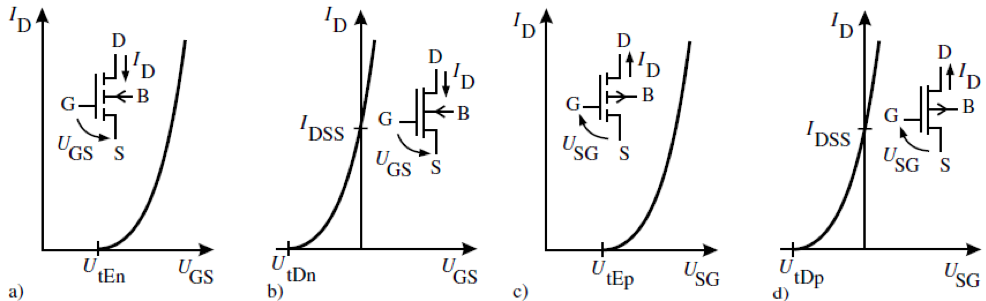
\includegraphics[height=2.4cm]{./images/MOSFETSteuerkennlinien.png}
            \end{minipage}
            \begin{minipage}[T]{9cm}
                a) n-Kanal Anreicherungs-Typ (selbstsperrend)\\
                b) n-Kanal Verarmungs-Typ (selbstleitend)\\
                c) p-Kanal Anreicherungs-Typ (selbstsperrend)\\
                d) p-Kanal Verarmungs-Typ (selbstleitend)\\
            \end{minipage}
                           
            \subsubsection{Berechnung des Drainstromes $I_D$}
            \begin{minipage}{13cm}
                $I_D = \begin{cases}
                0                       & $für $ V_{GS} \leqq V_{th}\\
                {\bf Sperrbereich}\\\\
                
                \beta\cdot(V_{GS} - V_{th})^2\cdot(1 + \lambda\cdot V_{DS})    &  $
                für $ 0\leqq V_{GS} - V_{th} \leqq V_{DS}\\
                {\bf Pentodenbereich} $ PB Sättigungsbereich $\\\\
                
                \beta\cdot(2(V_{GS}-V_{th})V_{DS} - V_{DS}^2)\cdot(1 + \lambda\cdot V_{DS}) &  $
                für $ 0\leqq V_{GS} - V_{th} \geqq V_{DS}\\
                {\bf Triodenbereich} $ TB linearer Bereich$
                
                \end{cases}$\\
                
                \begin{tabular}[t]{l l l}
                    $b$: Kanalbreite & $L$: Kanallänge & $\mu_n$: Leitfähigkeit Kanal\\
                    $\epsilon_{ox}$: Dielektrizität Oxidschicht & $\lambda$: Pinch-off-Konstante & $d_{ox}$: Oxiddicke\\
                    $V_{th}$: Threshold-Spannung & $\beta$: Steilheitsparameter & $K$: Steilheitskoeffizient
                \end{tabular}
            \end{minipage}
            \vrule \hspace{0.1cm}
            \begin{minipage}[T]{6cm}
                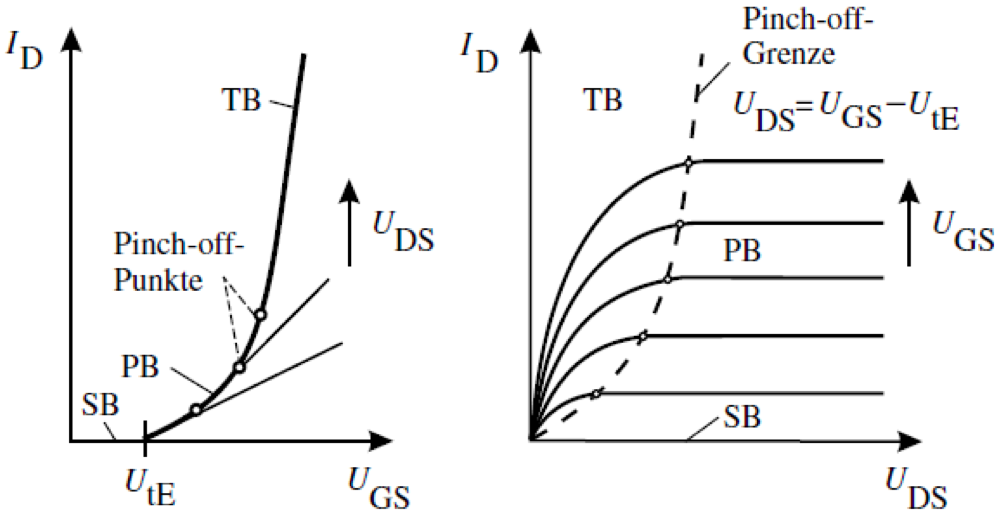
\includegraphics[width=6cm]{./images/MOSFET_IU_Kennlinie.png}\\
                \vspace{0.8cm}\\
                Steilheitsparameter \hspace{1mm}\fbox{$\beta = \frac{K}{2} = \frac{\mu_n \epsilon_{ox}}{2d_{ox}}\frac{b}{L}$}
            \end{minipage}\\
            
            \subsubsection{Kleinsignalmodell des MOSFET}
            \begin{minipage}[T]{10.5cm}
                Steilheit
                \hspace{29.3mm}\fbox{$S = g_m = 2\beta(V_{GS}-V_{th}) = \sqrt{4\beta\cdot I_D}$}\\
                Ausgangsleitwert
                \hspace{15.9mm}\fbox{$g_d = \beta\lambda(V_{GS}-V_{th})^2$}\\
                Drain-Source-Widerstand
                \hspace{3mm}\fbox{$r_{DS} = \frac{1}{\lambda\cdot I_{D0}}$}\\
                Gate-Source-Spannung
                \hspace{7mm}\fbox{$V_{GS} \cong \sqrt{\frac{I_D}{\beta}} + V_{th}$}
            \end{minipage}
            \begin{minipage}[T]{3.5cm}
                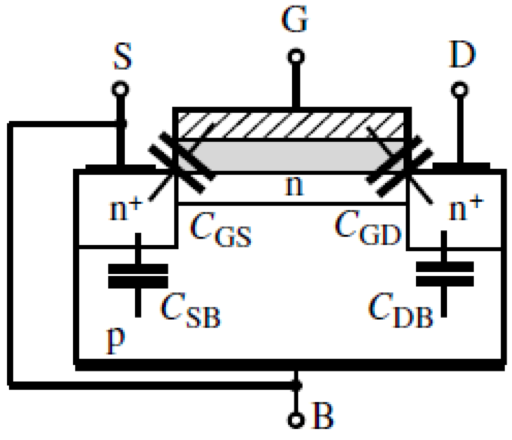
\includegraphics[width=3cm]{./images/MOSFET_Aufbau.png}
            \end{minipage}
            \begin{minipage}[T]{5cm}
                \includegraphics[width=5cm]{./images/MOSFET_Ersatzsch.png}
            \end{minipage}
\vspace{1mm}\hrule
            \subsubsection{Differenzverstärker}
            \begin{minipage}[T]{14cm}
                Ausgangswiderstand
                \hspace{10.6mm}\fbox{$r_{out} = R//r_{DS}$}\\
                Verstärkung
                \hspace{23.3mm}\fbox{$A_D = -\frac{S}{2} \cdot R$}\\
                Ausgansdifferenzspannung
                \hspace{1.7mm}\fbox{$V_{out_{diff}} = A \cdot V_{in_{diff}}$}
                
            \end{minipage}
            \begin{minipage}[T]{5cm}
                \includegraphics[height=4cm]{./images/MOSFET_Diffamp.png}
            \end{minipage}
\section{Referenzspannungen} 

\subsection{Verschiedene Arten der Rerferenzspannungserzeugung} 
	\begin{longtable}{|l|l|l|}
	\hline
		\begin{minipage}{4cm}
			\textbf{Einfachste "`Referenzspannungsquelle"'}
		\end{minipage}
	&
		\begin{minipage}{6cm}
			\includegraphics[width=6cm,trim=0 0 0 -5]{images/spannungsteiler}
		\end{minipage}
	&
		\begin{minipage}{8cm}
			\begin{equation*}
				S_{V_{DD}}^{U_{Ref}}=\frac{\frac{\Delta
				U_{Ref}}{U_{Ref}}}{\frac{\Delta V_{DD}}{V_{DD}}}=1
			\end{equation*}
			S: Sensitivität: Relative Änderung des Ausgangs zu Relativer Änderung des Eingangs
		\end{minipage}
	\\ \hline
		\begin{minipage}{4cm}
			\textbf{Dioden Referenz}
		\end{minipage}
	&
		\begin{minipage}{6cm}
			\includegraphics[width=6cm]{images/diodenReferenz}
		\end{minipage}
	&
		\begin{minipage}{8cm}
			\begin{gather*}
				U_{Ref}=U_{EB}=\frac{kT}{e}\ln{\frac{I}{I_{s}}} \notag\\
				\text{ für }V_{DD} \gg U_{EB}\\
				S_{V_{DD}}^{U_{Ref}}=\frac{1}{\ln{\frac{I}{I_{S}}}}<1
			\end{gather*}
		\end{minipage}
	\\ \hline
		\begin{minipage}{4cm}
			\textbf{MOSFET Referenz}
		\end{minipage}
	&
		\begin{minipage}{6cm}
			\includegraphics[width=2.5cm,trim=0 0 0 -5]{images/mosfetReferenz}
		\end{minipage}
	&
		\begin{minipage}{8cm}
			\begin{equation*}
				V_{REF}\approx \frac{R_{1}+R_{2}}{R_{2}}V_{GS}
			\end{equation*}
			\begin{equation*}
				V_{GS} \approx \text{ konst.}\quad\Leftrightarrow\quad V_{out} \text{ konst.}
			\end{equation*}
			$V_{GS}$ hat grosse Toleranzen $\Leftrightarrow$ eher unüblich
		\end{minipage}
	\\ \hline
		\begin{minipage}{4cm}
			\textbf{Bootstrap Referenz}
		\end{minipage}
	&
		\begin{minipage}{6cm}
			\includegraphics[width=6cm]{images/bootstrapReferenz}
		\end{minipage}
	&
		\begin{minipage}{8cm}
			\begin{gather*}
				I_{1}=I_{2} \\
				I_2 \cdot R = m \cdot  U_T \cdot \ln\left(\frac{I_1}{I_S}\right) \\
				U_{T}=\frac{kT}{q}
			\end{gather*}
				Stromspiegel (PTAT-Stromquelle) \\
				(PTAT: Proportional To Absolute Temperature)
			\end{minipage}
	\\ \hline
		\begin{minipage}{4cm}
			\textbf{Bandgap Referenz}
		\end{minipage}
	&
		\begin{minipage}{6cm}
			\includegraphics[width=6cm,trim=0 0 0 -5]{images/bandgapReferenz1}\\
			\includegraphics[width=6cm]{images/bandgapReferenz2}
		\end{minipage}
	&
		\begin{minipage}{8cm}
			Addition aus zwei Spannungen mit umgekehrten, 
			gleich grossen Temperatur-Koeffizienten:
			\begin{enumerate}
				\item Diodenspannung mit $-2 \frac{mV}{K}$ (hier: $U_{BE3}$)
				\item PTAT-Quelle mit $V_T=\frac{kT}{q} \Rightarrow +0.085 \frac{mV}{K}$
			\end{enumerate}

			\textbf{Herleitung:} \\
			Generell ist $I_C = B \cdot I_{BS} \left(e^{\frac{U_{BE}}{U_T}} -1 \right)
							\approx B \cdot I_{BS} \cdot e^{\frac{U_{BE}}{U_T}}$ \\
			Damit wird $\frac{I_{C1}}{I_{C2}}$ zu $e^{\frac{U_{BE1}-U_{BE2}}{U_T}}$ \\
			und $\Delta U_{BE} = U_{BE1}-U_{BE2} = U_T \ln\left(\frac{I_{C1}}{I_{C2}}\right)$ \\
			\\
			Ist das Verhältnis \smash{$\frac{I_{C1}}{I_{C2}}$} konstant, was beim Stromspiegel
			erfüllt ist, so hängt $\Delta U_{BE}$ wegen \smash{$U_T=\frac{k \cdot T}{q}$} nur 
			von der absoluten Temperatur $T$ ab ist somit eine PTAT-Quelle. \\
			\\
			Weil $I_{R3} \approx I_{R2}$ hängt auch $U_{PTAT}=I_{R3} \cdot R_3$ nur von der
			absoluten Temperatur $T$ und ist somit eine PTAT-Quelle. \\
			\\
			$U_{Ref} = U_{PTAT} + U_{BE3}$ ist also die Addition einer PTAT-Quelle und einer
			Diodenspannung und somit praktisch temperaturunabhängig mit 
			$U_{Ref} \stackrel{!}{\approx} 1,2V$. \\
			\\
			\textit{Oft als integrierte Bauteile erhältlich.}
		\end{minipage}
	\\ \hline
		\begin{minipage}{4cm}
			\textbf{Zenerdiode Referenz}
		\end{minipage}
	&
		\begin{minipage}{6cm}
			\includegraphics[width=6cm,trim=0 0 0 -5]{images/zenerReferenz}
		\end{minipage}
	&
		\begin{minipage}{8cm}
			Häufigste Spannung: $5,6V$ (minimaler Temperaturkoeffizient)
		\end{minipage}
	\\ \hline
\end{longtable}


\newpage
\section{Spannungsregler/Stromversorgung} 
	\subsection{Lineare Spannungsregler} 
		Für alle linearen Spannungsregler gilt: 
		\begin{equation*}
			P_{V}=(V_{E}-V_{a}) \cdot I_{a}
		\end{equation*}
		Einsatz für geringer Spannungsunterschied zwischen Eingangsspannung und der
		geregelten Ausgangsspannung \\
		
		\subsubsection{Qualitätsmasse}
			\begin{tabular}{l l}
				Relativer Stabilisierungsfaktor & $S' = \frac{\frac{\Delta U_e}{U_e}}
														{\frac{\Delta U_a}{U_a}}$ \\
				Temperaturkoeffizient & $TK_U = \frac{1}{U_a} \cdot \frac{dU_a}{dT}$ \\
				Dynamischer Ausgangswiderstand & $r_a = \frac{dU_a}{dI_a}$ \\
			\end{tabular} \\

\begin{longtable}{|l|l|l|}
	\hline
		\begin{minipage}{4cm}
			\textbf{Spannungs-stabilisierung mit Transistor}
		\end{minipage}
	&
		\begin{minipage}{6cm}
			\includegraphics[width=6cm]{images/transistorStabilisierung}
		\end{minipage}
	&
		\begin{minipage}{8cm}
			\begin{gather*}
				U_{A}=U_{Z}-U_{BE}\\
				R_{V}=\frac{U_{E}-U_{Z}}{I_{Z}+I_{B}}\\
				I_{B}=\frac{I_{C}}{B}\\
				I_{C} \approx I_E = I_L \\
				R_{i}\approx\frac{r_{Z}}{\beta} 
			\end{gather*}
			
			\begin{tabular}{ll}
				$U_{Z}$:&Z-Dioden-Spannung\\
				$I_{Z}$:&Strom durch die Z-Diode\\
				$R_{i}$:&Innenwiderstand der Schaltung\\
				$r_{Z}$:&dyn. Innenwiderstand der Z-Diode\\
				$B$:&Gleichstromverstärkung \\
				$\beta$:&Dynamische Verstärkung \\
			\end{tabular}
		\end{minipage}
	\\ \hline
		\begin{minipage}{4cm}
			\textbf{Lineare Regler}
		\end{minipage}
	&
		\begin{minipage}{6cm}
			\includegraphics[width=6cm,trim=0 0 -5 -5]{images/linearRegler}
		\end{minipage}
	&
		\begin{minipage}{8cm}
			\begin{gather*}
				U_a = \left( 1+ \frac{R_1}{R_2} \right) \cdot U_{ref}
			\end{gather*}
			Erhältlich als integrierte Regler, z.B. 78xx \\
			Spannungsabfall $\approx 2V$ \\
			\\
			Low-Dropout-Regler (LDO): PMOS-FET anstatt Transistor \\
		\end{minipage}
	\\ \hline
		\begin{minipage}{4cm}
			\textbf{Lineare Regler mit einstellbarer Ausgangsspannung}
		\end{minipage}
	&
		\begin{minipage}{6cm}
			\includegraphics[width=6cm, trim=0 0 0 -5]{images/einstellbarStabilisierung}
		\end{minipage}
	&
		\begin{minipage}{8cm}
			Adjust-Pin (ADJ) zum Anschluss der externen Widerstände $R_1,R_2$
			\begin{gather*}
				U_a = U_{R_1} + U_{R_2} = U_{ref} + R_2 \cdot 
				\left(\frac{U_{ref}}{R_1} + I_{adj}\right) \\
				\text{für }I_{adj} \ll I_{R_1} \text{gilt:} \\
				U_a = U_{ref} \cdot \left(1+\frac{R_2}{R_1}\right)
			\end{gather*}
		\end{minipage}
	\\ \hline
\end{longtable}

\subsection{Schaltregler}
	\subsubsection{Grundprinzip}
		Energie wird in verlustarmem Element zwischengespeichert und auf gewünschter
		Spannung stabilisiert. Als Energiespeicher kommen in Frage: \textbf{Kondensatoren}
		für kleine Leistungen und \textbf{Spulen} für mittlere bis grosse Leistungen.
		Übliche Schaltfrequenzen liegen im Bereich von $200kHz$. \\
		
		Energie wird im Magnetfeld gespeichert: $E_L = \frac{L}{2} \cdot i_L^2$ \\
		Spannung über Spule bewirkt Stromänderung: $I_L = \frac{1}{L} \int V_L(t) \, dt$ 
		oder $V_L = L \cdot \frac{d}{dt} I_L(t)$\\
		Kondensator am Ausgang stabilisiert Spannung ($E_C = \frac{1}{2} \cdot C \cdot U^2$)\\
		
		\begin{minipage}{8cm}
			\textbf{Abwärtswandler} (Step-Down, Buck Converter) \\
			\includegraphics[width=6cm]{images/buckConv} \\
			\textbf{Invertierender Wandler} (Inverting) \\
			\includegraphics[width=6cm]{images/invConv} \\
		\end{minipage}
		\begin{minipage}{8cm}
			\textbf{Aufwärtswandler} (Step-Up, Boost Converter) \\
			\includegraphics[width=6cm]{images/boostConv} \\
			\textbf{Sperrwandler} (Flyback Converter) \\
			\includegraphics[width=6cm]{images/flybackConv}
		\end{minipage}

\subsection{Aufwärtswandler}
	\begin{minipage}{6cm}
		\includegraphics[width=6cm]{./images/boost-Verhalten}
	\end{minipage}
	\begin{minipage}{12cm}
		\begin{align*}
			&\text{Ladephase (Switch on)} & \Delta I_{L_{on}} & = \frac{1}{L} \cdot U_{in} \cdot t_{on} \\
			&\text{Entladephase (Switch off)} & \Delta I_{L_{off}} & = \frac{1}{L} \cdot \left(U_{in}-U_{out}\right) \cdot t_{off} \\
			&\text{Gleichgewicht} & \Delta I_{L_{on}} & = -\Delta I_{L_{off}} \\
			&\text{Ausgangsspannung}	& U_{out} & = U_{in} \cdot \left( 1+\frac{t_{on}}{t_{off}}\right)
		\end{align*}
	\end{minipage}

\subsection{Abwärtswandler}
	\begin{minipage}{6cm}
		\includegraphics[width=4cm]{./images/buck-Verhalten}
	\end{minipage}
	\begin{minipage}{12cm}
		\begin{align*}
			&\text{Schalter geschlossen} & \Delta I_{L_{on}} &= \int_{0}^{T_i} (U_e - U_a) dt = \frac{1}{L} \cdot (U_e - U_a) \cdot T_i \\
			&\text{Schalter offen} & \Delta I_{L_{off}} &= \int_{T_i}^{T_s}(U_a + U_{F_0} dt = \frac{1}{L} \cdot (U_a - U_{F_0}) \cdot (T_s - T_i) \\
			&\text{Bilanz} & U_a &= \frac{T_i}{T_s} \cdot U_e - \left(1-\frac{T_i}{T_s} \right) \cdot U_{F_0} \approx \frac{T_i}{T_s} \cdot U_e
		\end{align*}
	\end{minipage}
	
\subsection{Invertierender Wandler}
	\begin{minipage}{6cm}
		\includegraphics[width=4cm]{./images/invWandler-Verhalten}
	\end{minipage}
	\begin{minipage}{12cm}
		\[ U_a = -\frac{T_i}{T_s} \cdot U_e \]
	\end{minipage}

\subsection{Ladungspumpen}
	Prinzip: Regelung der Ausgangsspannung durch Ändern der Schaltfrequenz \\
	\begin{minipage}{5cm}
		\includegraphics[width=4cm]{./images/ladungspumpe-normal}
	\end{minipage}
	\begin{minipage}{5cm}
		\includegraphics[width=4cm]{./images/ladungspumpe-inv}
	\end{minipage}
	\begin{minipage}{6cm}
		\begin{align*}
			\Delta U_a &= \frac{U_e - U_a}{1 + \frac{C_L}{C_1}} \\
			\Delta Q &= C_L \cdot \Delta U_a &= \frac{C_L \cdot C_1}{C_L + C_1} (U_e - U_a) \\
			I_a &= I_e = \frac{\Delta Q}{T_s} &= \frac{C_L \cdot C_1}{C_L + C_1} \frac{U_e - U_a}{T_s}
		\end{align*}
	\end{minipage}
	
\subsection{Effizienzsteigerung}
	\subsubsection{MOSFET statt Diode}
		\includegraphics[width=12cm]{images/effizient1}
		\begin{itemize}
		\begin{minipage}{8cm}
 		 	\item Diode hat Spannungsabfall
  			\begin{itemize}
    			\item Silizium-Diode: 0.7V
   				\item Schottky-Diode: 0.3V
    			\item MOSFET hat "`nur"' On-Widerstand $R_{DS_{on}}$
			\end{itemize}
		\end{minipage}
		\begin{minipage}{8cm}
			\item Umschalten vom Substratpotential beim Längstransistor nötig
   			\begin{itemize}
     			\item Synchronous rectifier
    		\end{itemize}
		\end{minipage}
		\end{itemize}
\section{Oszilatoren}
\subsection{Typen}
	\begin{center}
		\includegraphics[width=11cm]{images/osziTypen.png}
	\end{center}
\subsection{Rechteckgenerator}
	\begin{multicols}{3}
		\includegraphics[width=6cm]{images/osziRechteck.png}
		\columnbreak
		
		\includegraphics[width=6cm]{images/osziRechteckSignal.png}
		\columnbreak
		
		$V_{T+}=V_{outMAX}\cdot\frac{R_2}{R_2+R_3}$\\
		$V_{T-}=V_{outMIN}\cdot\frac{R_2}{R_2+R_3}$\\
		$V_c(t)=V_{T-}+\left(V_{outMAX}-V_{T-}\right)\left(1-e^{\frac{-t}{R_1\cdot
		C_1}}\right)$\\
		$f=\frac{1}{T}=\frac{1}{2R_1C_1 ln \frac{R_3+2R_2}{R3}}$\\
		wenn: $R2 = 0.86 \cdot R_3$ dann $ln\frac{R_3 +2 \cdot 0.86 \cdot R_3}{R_3}=ln
		\left( 2.72 \right) = 1$\\
		$\Longrightarrow f=\frac{1}{2\cdot R_1C_1}$
	\end{multicols}
\subsection{Dreieck Rechteck Generator}
	\begin{multicols}{3}
		\begin{center}
			\includegraphics[width=3.5cm]{images/osziDreieckRechteckBlock.png}\\
		\end{center}
		\includegraphics[width=6cm]{images/osziDreieckRechteck.png}
		\columnbreak
		
		\includegraphics[width=6cm]{images/osziDreieckRechteckSignal.png}
		\columnbreak
			
		$V_2\left(t\right)=-\frac{1}{R_1C}\int V_1\left(t\right)dt+V_{2 Anfang}$\\
		$V_H=2\left|V_T\right|=\left(V_{outMAX}-V_{outMIN}\right)\frac{R_2}{R_3}$\\
		$T=\frac{2\cot V_H \cdot R_1C}{V_{outMAX}}$\\
	\end{multicols}
\subsection{Ringoszilatoren}
	\begin{multicols}{3}
	 	\includegraphics[width=6cm]{images/osziRing.png}	
		\columnbreak
		
		\includegraphics[width=6cm]{images/osziRingSignal.png}	
		\columnbreak
		
		\includegraphics[width=6cm]{images/osziRingCMOS.png}
	\end{multicols}
\subsection{VCO (voltage controlled oscialltors)}
	\begin{multicols}{2}
		\includegraphics[width=9cm]{images/osciVCO.png}
		\columnbreak
		
		$OP4$ bildet mit $R_1$ und $R_2$ einen Schmitt-Trigger.\\
		$OP3$ bildet mit $R$ und $C$ ein Integrator.\\
		$f_{osc}=\frac{R_2}{4\cdot R_1}\cdot \frac{1}{RC}\cdot
		\frac{V_{ctrl}}{\left|V_{out}\right|}=K_{VCO}\cot V_{ctrl}$\\
	\end{multicols}
\subsection{LC-Oszillator}
	\begin{multicols}{3}
		\includegraphics[width=6cm]{images/osziLC.png}\\
		Aufbau eine Colpitts-Oszillators
		\columnbreak
		
		$T\left(s\right)=\frac{-A}{1+sR\left(C_1+C_2\right)+s^2LC_2+s^3RLC_1C_2}$\\
		$s=j\omega$ und $\Im{T\left(j\omega\right)}=0$ ergeben $\omega_0$\\
		$\omega_0=\frac{1}{\sqrt{L\frac{C_1 C_2}{C_1+C_2}}}$\\
		\columnbreak
		
		Aus $T\left(j\omega\right)=1$ ergeben die Amplituden = und Anschwingbedignugnen
		$\geq$
		$A=\frac{C_2}{C_1}$ bzw. $A\geq\frac{C_2}{C_1}$
	\end{multicols}
\subsection{Quarz-Oszilator}
	\begin{multicols}{3}
		\includegraphics[width=3cm]{images/osziCrystal.png}
		\columnbreak
		
		$Z_{Xtal}\left(\omega\right)=\frac{\left(R+sL+\frac{1}{sC}\right)\frac{1}{sC_0}}{R+sL+\frac{1}{sC}+\frac{1}{sC_0}}$\\
		\\
		Wenn $R \ll \omega L$:\\
		$Z_{Xtal}\left(\omega\right)=\frac{s^2LC+1}{s\left(s^2LCC_0+C+C_0\right)}$\\
		\columnbreak
		
		f\"ur $Z\left(s\right)=jX\left(\omega\right)$:\\
		\\
		$X\left(\omega\right)=-\frac{1}{\omega C_0}\cdot \frac{\omega^2 -
		\omega_s^2}{\omega^2-\omega^2_P}$
	\end{multicols}

\newpage
\section{Idiotenseite}
\input{idiotenseite/trigo/trigoInclude}

\end{document}
